\documentclass[uplatex,dvipdfmx]{jlreq}
\usepackage[fleqn,tbtags]{mathtools}
\usepackage{jlreq-deluxe}
\usepackage{geometry}
\usepackage{booktabs}
\usepackage{hyperref}
\usepackage[noalphabet]{pxchfon} % must be after otf package
\usepackage{stix2} %欧文＆数式フォント
\usepackage[fleqn,tbtags]{mathtools} % 数式関連 (w/ amsmath)
\usepackage{url}
\usepackage{here}
\geometry{left=20mm,right=20mm,top=25mm,bottom=25mm}

\title{作業ログ\\ \large プロジェクト名: [加速度センサーを用いた身体動作による輪唱制御システムの構築と視覚フィードバック効果]}
\author{報告者: 早川　和輝}
\date{報告日: 2026年6月17日}

\begin{document}
\maketitle

\section{進捗サマリー(要約)}
\begin{itemize}
    \item 全体進捗率: [75\%]
    \item マイルストーン達成状況: [達成]
    \item 主要成果:
    \begin{itemize}
        \item 成果1: テンポ変更処理の完成．100〜180bpmを20bpm刻みの5段階(0〜4)で切り替え，再生途中でも即時に反映できるようにした．
        \item 成果2: 同期用Arduinoとの連携を無線(WiFiのUDPブロードキャスト)で実装．再生開始・輪唱開始・テンポ・停止の各コマンドを受信できるようにした．
        \item 成果3: カエルの歌の輪唱を，楽器1台の中で2声部に重ねる方式で実装．音楽開始の合図と輪唱開始の合図を分離した．
        \item 成果4: 音階に連動してサーボモーター6機が動く処理を実装(ド・レ・ミ・ファ・ソ・ラの6音をサーボ6機に1対1で割当)．
        \item 成果5: Processingの可視化を，周波数スペクトル(FFT)から音の時間波形の表示へ変更．
    \end{itemize}
    \item 重大課題(影響度:無し): なし
\end{itemize}

\section{作業ログ(詳細トラッキング)}
\begin{table}[H]
    \centering
    \small
    \begin{tabular}{lp{1.5cm}p{1.5cm}llp{2.5cm}p{3cm}}
        \toprule
        作業項目 & 開始日 & 完了日 & 状態 & 進捗率 & 依存関係・ブロッカー & コメント \\
        \midrule
        テンポを変更させる処理の追加 & [6/8] & [6/15] & 完了 & 100\% & なし & 100〜180bpmの5段階(20刻み)を実装．再生途中の即時変更にも対応． \\
        同期との連携(無線通信) & [6/11] & [6/17] & 進行中 & 80\% & 同期班の送信仕様 & WiFiのUDPブロードキャスト受信を実装．コマンド('A','B','0'〜'4','X')の取り決めを定義． \\
        輪唱(カエルの歌)の実装 & [6/13] & [6/17] & 進行中 & 90\% & なし & 楽器1台の中で2声部を重ねる方式で実装．'A'で主旋律，'B'で2声目が入る． \\
        サーボモーターの音階連動 & [6/9] & [6/16] & 完了 & 100\% & なし & 6音をサーボ6機に1対1で割当．鳴っている声部に対応するサーボが動く． \\
        波形表示への変更 & [6/14] & [6/15] & 完了 & 100\% & なし & Processingの可視化をFFTから時間波形へ変更． \\
        \bottomrule
    \end{tabular}
\end{table}

\section{担当箇所の計画前のGCと現在のGC}
担当箇所である「楽器演奏実装」における，当初計画時（計画前）のガントチャート（GC）の予定と，現在の進捗・変更状況の比較である．
\begin{table}[H]
    \centering
    \small
    \begin{tabular}{lp{4cm}p{4cm}l}
        \toprule
        タスク名 & 計画前のGC（予定期間） & 現在のGC（実績・修正期間） & 進捗状態 \\
        \midrule
        楽譜作成・Hz出力 & [5/23 $\sim$ 5/25] & [5/23 $\sim$ 5/23] & 完了 \\
        バイオリンの音色作成 & [5/29 $\sim$ 6/6] & [5/25 $\sim$ 5/27] & 完了 \\
        ギロの音色作成 & [5/29 $\sim$ 6/6] & [5/27 $\sim$ 6/6] & 完了 \\
        ArudinoとProcessingの連携 & [6/3 $\sim$ 6/7] & [6/3 $\sim$ 6/7] & 完了 \\
        音の動作確認 & [6/5 $\sim$ 6/9] & [6/5 $\sim$ 6/9] & 完了 \\
        テンポを変更させる処理の追加 & [6/8 $\sim$ 6/13] & [6/8 $\sim$ 6/15] & 完了 \\
        同期との連携 & [6/11 $\sim$ 6/17] & [6/11 $\sim$ 6/17] & 進行中 \\
        サーボモーターの動作確認 & [6/9 $\sim$ 6/13] & [6/9 $\sim$ 6/16] & 完了 \\
        \bottomrule
    \end{tabular}
\end{table}\begin{figure}[H]
    \centering
    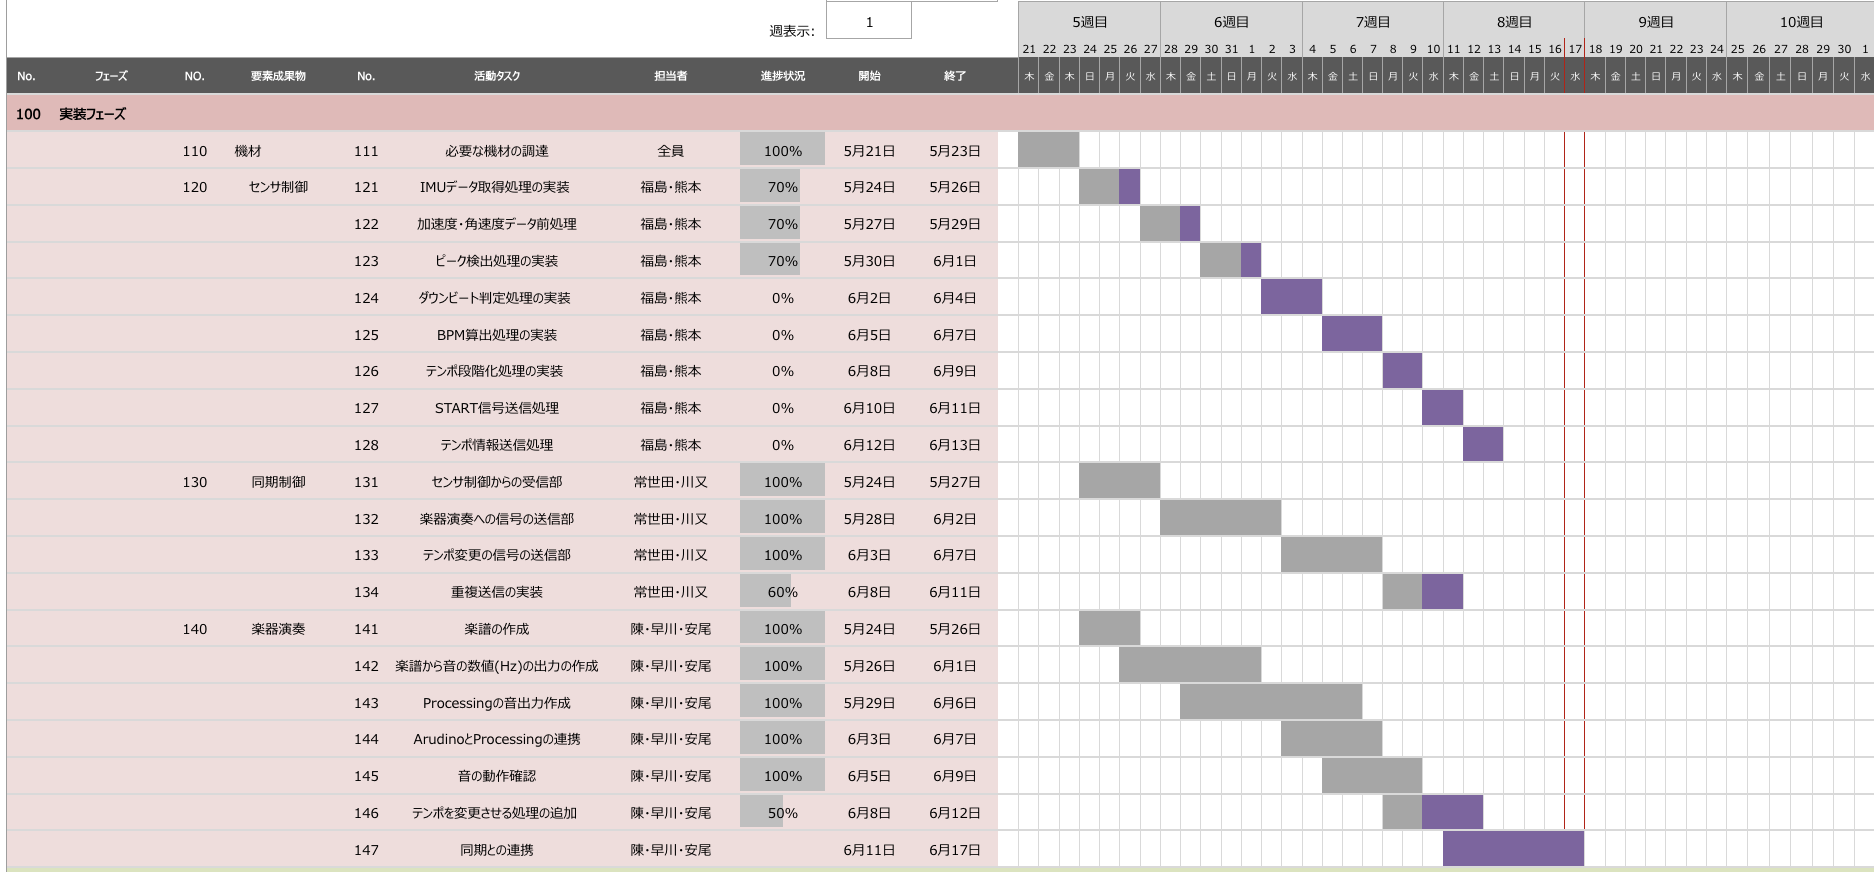
\includegraphics[width=0.8\textwidth]{ganto3.png}
    \caption{ガントチャート}
\end{figure}

\section{日ごとの作業時間と作業内容}
今週実施した日ごとの具体的な作業時間および対応内容の詳細です．
\begin{table}[H]
    \centering
    \small
    \begin{tabular}{lll}
        \toprule
        日付 & 作業時間 & 作業内容 \\
        \midrule
        {}[6/11] & [1.5時間] & 無線通信(WiFi)方式の調査と，同期コマンド仕様の設計． \\
        {}[6/13] & [2.0時間] & 輪唱(1台の中で2声部を重ねる方式)の実装． \\
        {}[6/14] & [1.5時間] & Processingの可視化を波形表示へ変更． \\
        {}[6/15] & [2.0時間] & テンポ5段階の実装と，再生途中での変更の動作確認． \\
        {}[6/16] & [1.5時間] & サーボの音階連動処理の実装． \\
        {}[6/17] & [1.5時間] & 全体の結合と動作確認． \\
        \midrule
        \textbf{合計} & \textbf{[10.0時間]} & \\
        \bottomrule
    \end{tabular}
\end{table}

\section{課題管理}
\begin{table}[H]
    \centering
    \small
    \begin{tabular}{p{3cm}p{3cm}llp{3cm}ll}
        \toprule
        課題 & 発生原因 & 影響度 & 優先度 & 対策 & 期限 & 状態 \\
        \midrule
        同期班との通信仕様の整合 & 送信側(同期班)のバイト符号化と受信側の取り決めが未統一 & 中 & 高 & コマンド仕様(A/B/0〜4/X，UDPポート)を文書化し同期班と擦り合わせる & [6/18] & 進行中 \\
        テンポ段階数の整合 & センサー班のテンポ段階数と本実装(5段階)が異なる可能性 & 中 & 中 & 段階数の対応表を共有し統一する & [6/18] & 進行中 \\
        実機での通信遅延・音ズレ & 無線通信の遅延が合奏の同期精度に影響する可能性 & 中 & 中 & 実機で遅延を測定し，許容範囲に収まるか確認する & [6/20] & 未着手 \\
        \bottomrule
    \end{tabular}
\end{table}
\vspace{0.5em}
\noindent ※影響度=プロジェクトへのインパクト，優先度=対応の緊急性

\section{AI 利用状況と検証(再現性重視)}
\subsection{利用内容}
\begin{itemize}
    \item 利用目的: \LaTeX による作業ログのテンプレート作成
    \item  入力(プロンプト要旨):
    \begin{itemize}
        \item 指定された作業ログのテンプレート項目の生成を依頼 ．
    \end{itemize}
    \item  出力概要:
    \begin{itemize}
        \item テンプレートの構成のコンパイル可能な作業ログの\LaTeX ソースコード ．
    \end{itemize}
\end{itemize}

\subsection{検証方法}
\begin{itemize}
    \item  検証手法: 生成された\LaTeX ソースコードの構造確認およびコンパイル検証
    \item  参照資料: 提供された作業ログテンプレートPDF
    \item  検証手順:
    \begin{enumerate}
        \item 生成されたコードのセクション構成が，テンプレート項目を漏れなく満たしているか目視で確認．
        \item \LaTeX 環境において実際にコンパイルを行い，エラーを吐かずに正しくPDFが生成されるかを確認．
    \end{enumerate}
\end{itemize}

\section{次回計画}
\begin{itemize}
    \item  目標: [同期班との通信仕様の統一と，実機での全体結合・音ズレ検証]
    \item  達成基準: [同期用Arduinoからの無線コマンドで全楽器が再生・輪唱・テンポ変更でき，実機で音ズレが許容範囲に収まること]
    \item  期限: [6/24]
\end{itemize}

\section{その他}

\end{document}
